\documentclass[11pt]{article}

\usepackage[letterpaper,bindingoffset=0.2in,
            left=1in,right=1in,top=1in,bottom=1in,
            footskip=.25in]{geometry}

\usepackage{hyperref}
	\hypersetup{
			colorlinks=true,
			linkcolor=black,
			filecolor=magenta,      
			urlcolor=blue,
	}
	
\usepackage{graphicx}
	\graphicspath{ {images/} }
	
\usepackage{subcaption}
	
\begin{document}


\title{COMP SCI 5401 FS2017 Assignment 1c}
\author{Stuart Miller\\\href{mailto:sm67c@mst.edu}{sm67c@mst.edu}}
\maketitle


\section{Overview}\label{sect:overview}

Assignment 1c presented a great many parameters to test. As more techniques are introduced, it becomes more and more difficult to distinguish a genuinely "`good"' parameter value as one can never be entirely sure if it was solely one value that resulted in a change in fitness landscape, a combination of multiple values, or perhaps the order of calls to the random number generator came out more favorably. Therefore, in this assignment, it has been attempted to isolate parameters being tested and pick favorable and reasonably values to the parameters not immediately relevant.

As a precursor, the entirety of this assignment will make use of n-point crossovers and random reset mutations. Although other operators are implemented in the codebase, these two have been set to be self-adaptive in Bonus 2. For consistency with the runs in the Bonus section, even when self-adaptability is turned off, the analysis will still use only these two operators. For initial values and non adaptive states, the operators will be fixed at three crossover points and a 12\% mutation chance. These are values that were determined to be beneficial in Assignment 1b. Furthermore, survival strategy will always be set to comma \((\mu,\lambda)\) and selection will be k-tournaments with moderate selective pressure.


\section{Penalty Coefficient}\label{sect:penalty}

To test the penalty coefficient, two control sets were run where invalid placements were solved by random replacements and then a repair. The penalty function was then implemented, with static weights of 1.0, 2.0, and 5.0, respectively.

As the graph in Figures \ref{fig:penaltyset1}, \ref{fig:penaltyset2}, and \ref{fig:penaltyset3} all show, the penalty weight functions shows significantly lower fitness values than other methods. This is to be expected for intermediate solutions, but the best solution shouldn't have any penalty. Additionally, the fact that the different weights returned the same max fitness shows that this may not be an optimal strategy for this problem. It is worth noting that numerous evolutionary strategy were tried and this combination yielded the best and most consistent results.

In all three data sets, each penalty weight averaged to be more or less the same final value. This similarity between data sets is likely due to the fact that in all instances, invalid solutions are VERY easy to come by (and can consequently be resolved small alterations from the repair function). Regardless of the complexity of the shapes, penalizable values are just as likely.

\begin{figure}[h]
\begin{minipage}{.5\textwidth}
  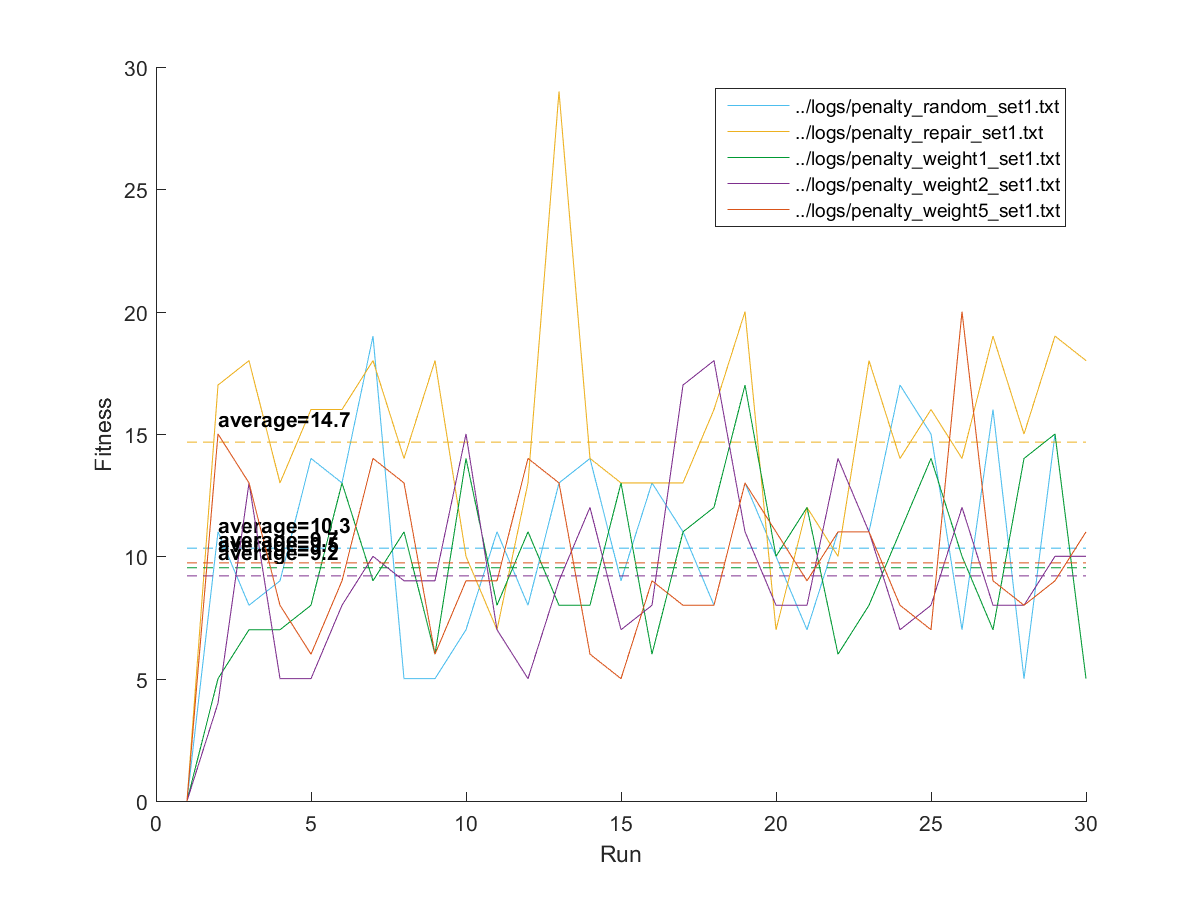
\includegraphics[width=3.25in]{assn1c_graph_penalty_set1.png}
  \captionof{figure}{Penalty Weights, 50Shapes.txt}
  \label{fig:penaltyset1}
\end{minipage}%
\begin{minipage}{.5\textwidth}
  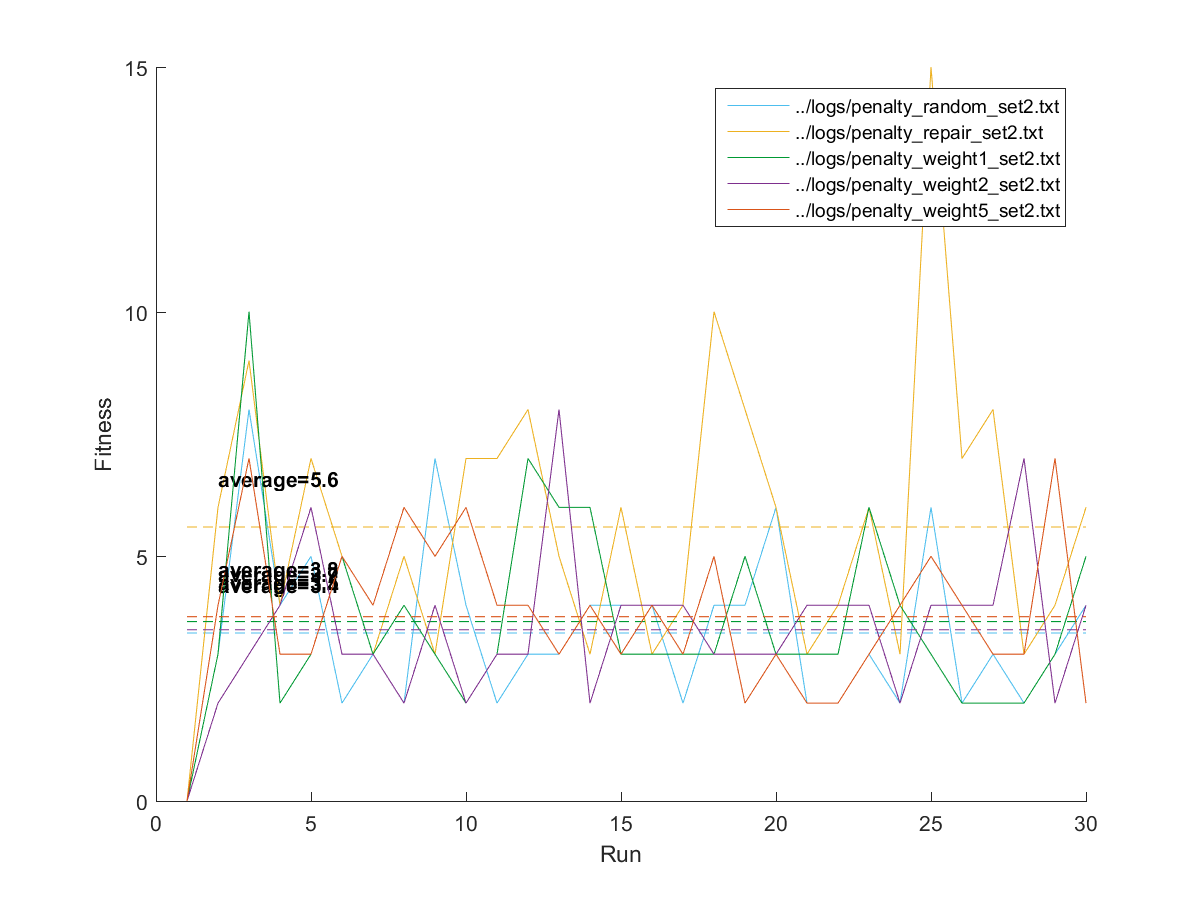
\includegraphics[width=3.25in]{assn1c_graph_penalty_set2.png}
  \captionof{figure}{Penalty Weights, 100Shapes.txt}
  \label{fig:penaltyset2}
\end{minipage}
\end{figure}
\begin{figure}[h]
	\centering
  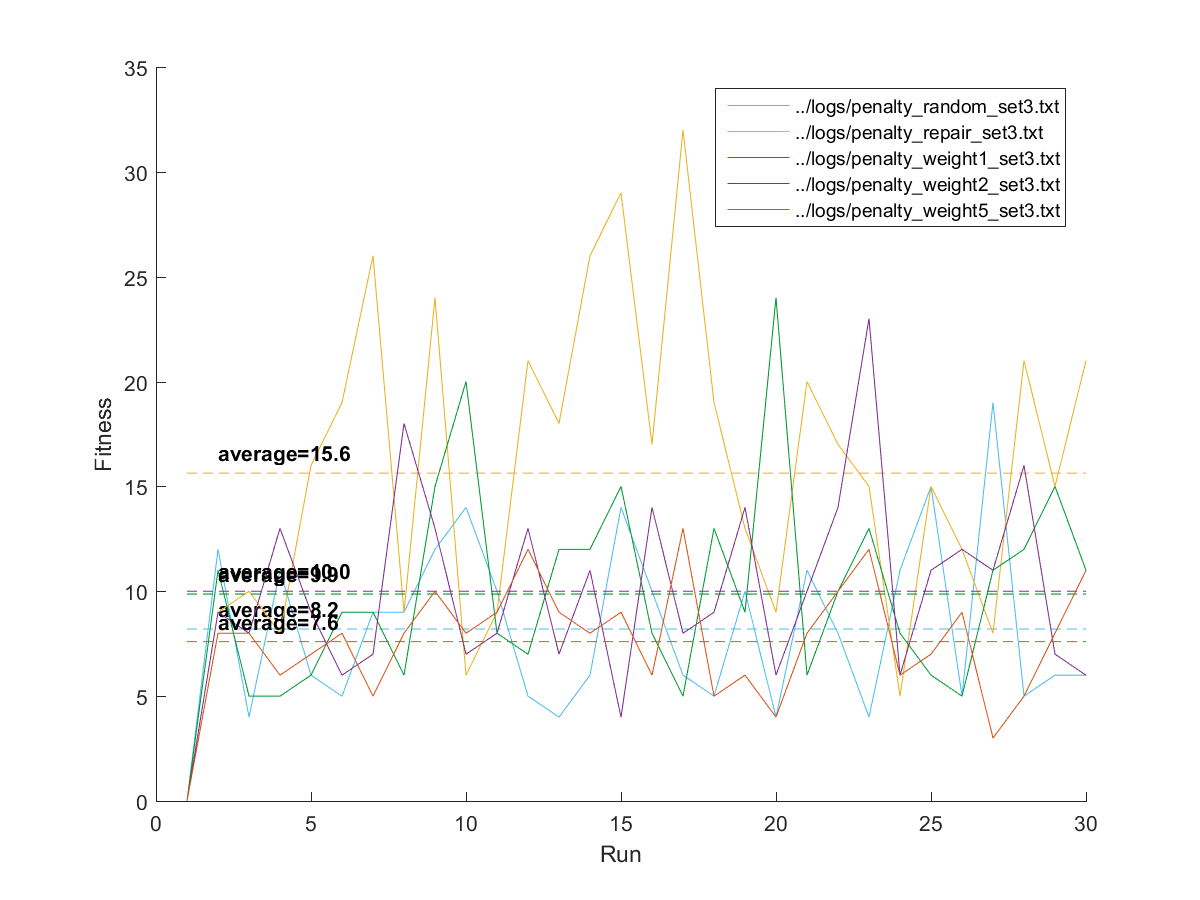
\includegraphics[width=3.25in]{assn1c_graph_penalty_set3.png}
  \captionof{figure}{Penalty Weights, 100ShapesComplex.txt}
  \label{fig:penaltyset3}
\end{figure}


\section{Self-Adaptive Parameter}\label{sect:selfadaptive}

To test self-adaptability, the number of crossover points \textit{n} was set to be adaptable. For offspring created, there was an equivalent random chance of inheriting each parent's \textit{n}. Additionally, \textit{n} had a small chance to mutate (equivalent to the genetic mutation rate) by $\pm$1. For analysis, \textit{n} was averaged across all member of the population for each generation and then logged.

As it was determined in Section \ref{sect:penalty}, the penalty function yields no great benefit for this problem, so the repair function method was used here instead. The other parameters were kept the same as in section \ref{sect:penalty}.

As figures \ref{fig:crossoverset1}, \ref{fig:crossoverset2}, and \ref{fig:crossoverset3} all show, allowing crossovers to self-adapt has a significant improvement on the average best fitness. It is also interesting to worth noting that while each instance started at three crossover points, some runs took this number higher, and some drove it lower. Examining the log (located in the ./logs/ directory) shows no consistent trend. It can only be assumed that each run's random initialization took it to a different area of the fitness landscape where more or less crossovers were desirable.

There is no distinct difference between the three data sets; self-adaptivity always proved beneficial. In fact, the difference between the two was nearly the same each time. This is likely due to the fact that each instance of this problem has such a variable fitness landscape, that allowing the recombination to vary itself more (by increasing the number of crossovers) allowed each run to exploit its particular fitness landscape.

\begin{figure}[h]
\begin{minipage}{.5\textwidth}
	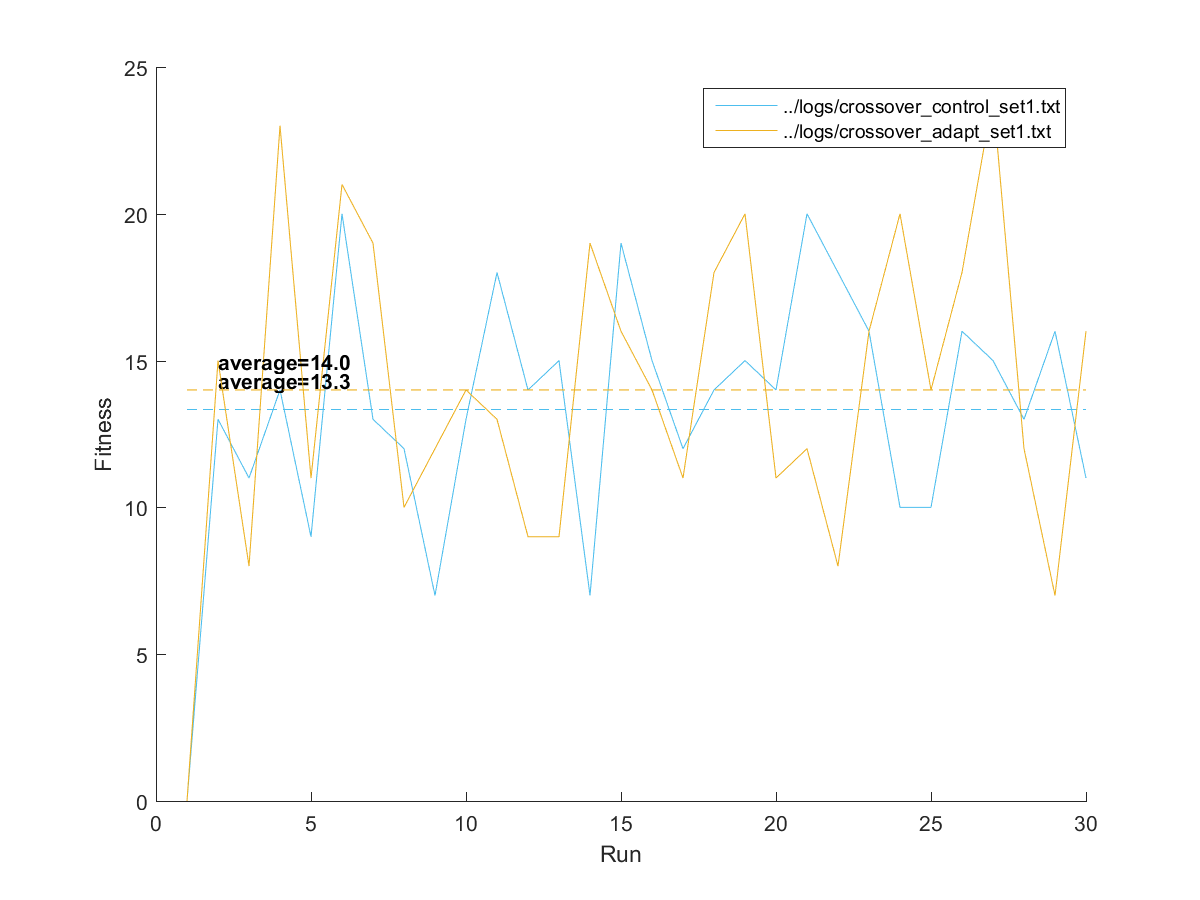
\includegraphics[width=3.25in]{assn1c_graph_crossover_adapt_set1.png}
  \captionof{figure}{Adaptive Crossovers, 50Shapes.txt}
  \label{fig:crossoverset1}
\end{minipage}%
\begin{minipage}{.5\textwidth}
  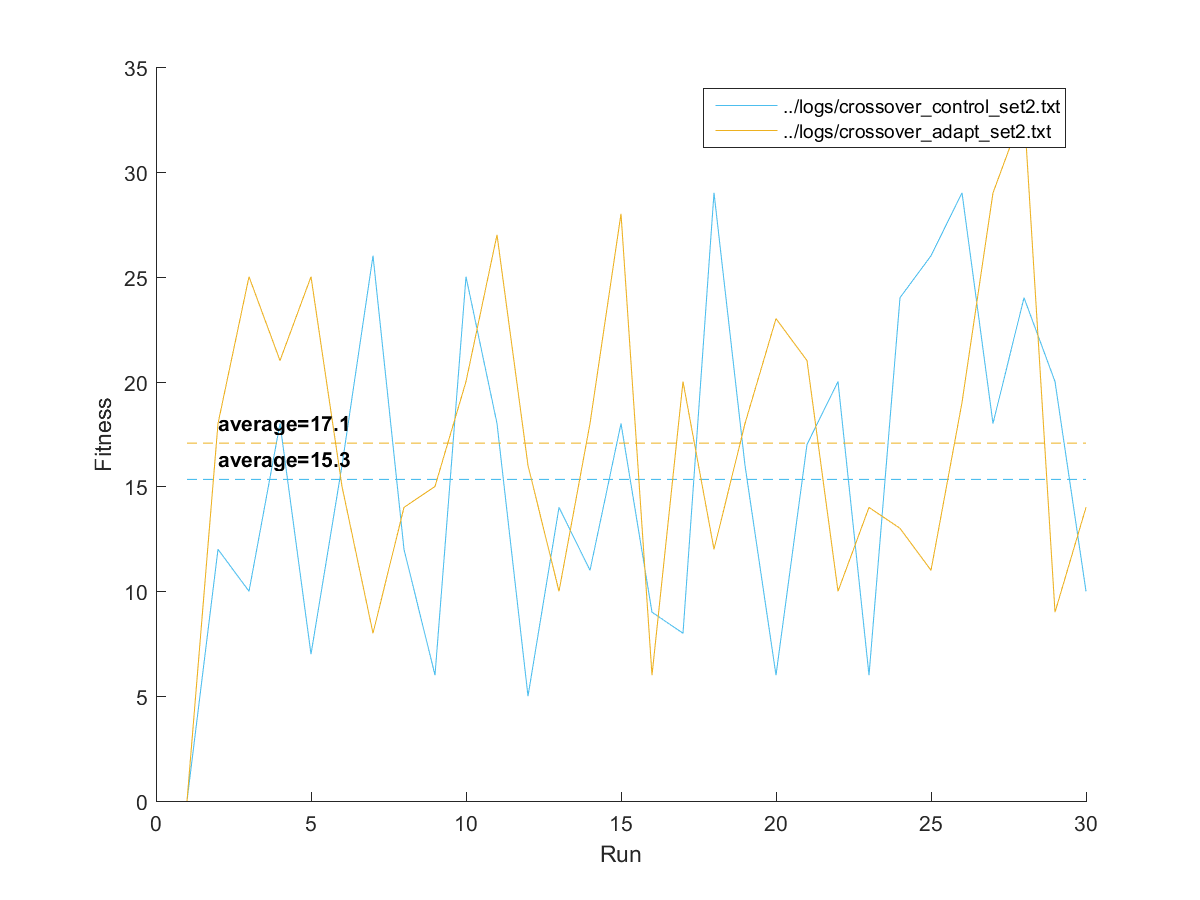
\includegraphics[width=3.25in]{assn1c_graph_crossover_adapt_set2.png}
  \captionof{figure}{Adaptive Crossovers, 100Shapes.txt}
  \label{fig:crossoverset2}
\end{minipage}
\end{figure}
\begin{figure}[h]
	\centering
  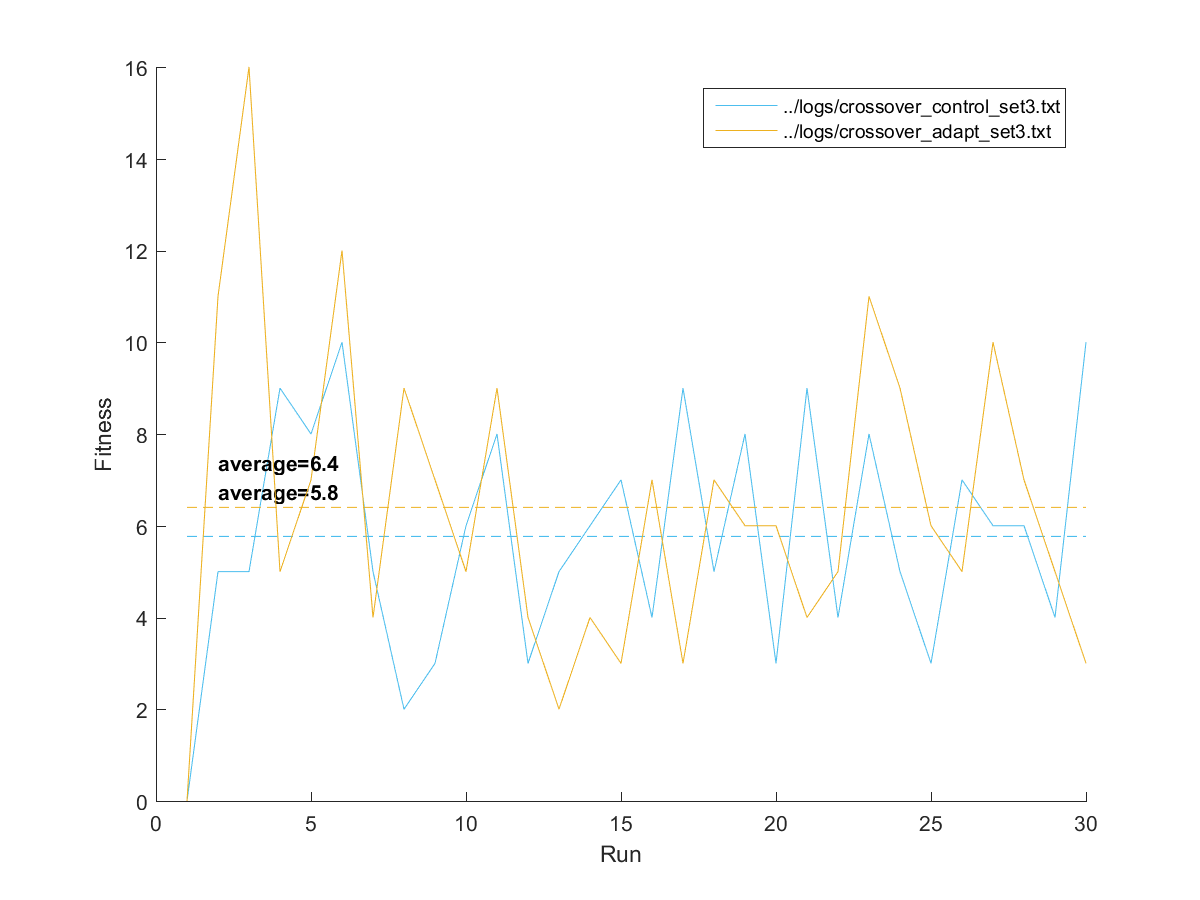
\includegraphics[width=3.25in]{assn1c_graph_crossover_adapt_set3.png}
  \captionof{figure}{Adaptive Crossovers, 100ShapesComplex.txt}
  \label{fig:crossoverset3}
\end{figure}


\section{Box Plots and Statistical Analysis}\label{sect:boxesandstats}

Box plots were generated for each test run graphed above. However, since this totals to a rather large number of boxplots, they have not all been pictured in this report. A full listing of box plots can be viewed in ./doc/images/assn1c\_boxplot\_*.png.

In Figures \ref{fig:boxplot1} and \ref{fig:boxplot2} box plots are shown for the first data set. It can be observed that the resulting populations are as to be expected, with an upper bound having the best fitness and the remaining population distributed below. It is worth noting that with the self-adaptive crossovers, the distribution tends to skew more towards the maximum. This is likely due to the fact that, as shown in Section \ref{sect:selfadaptive}, self-adaptivity pushes the population closer to a better fitness solution.

A statistical analysis was also run (Figures \ref{fig:statanal1} and \ref{fig:statanal2}) which further illustrates this finding.

\begin{figure}[h]
\begin{minipage}{.5\textwidth}
  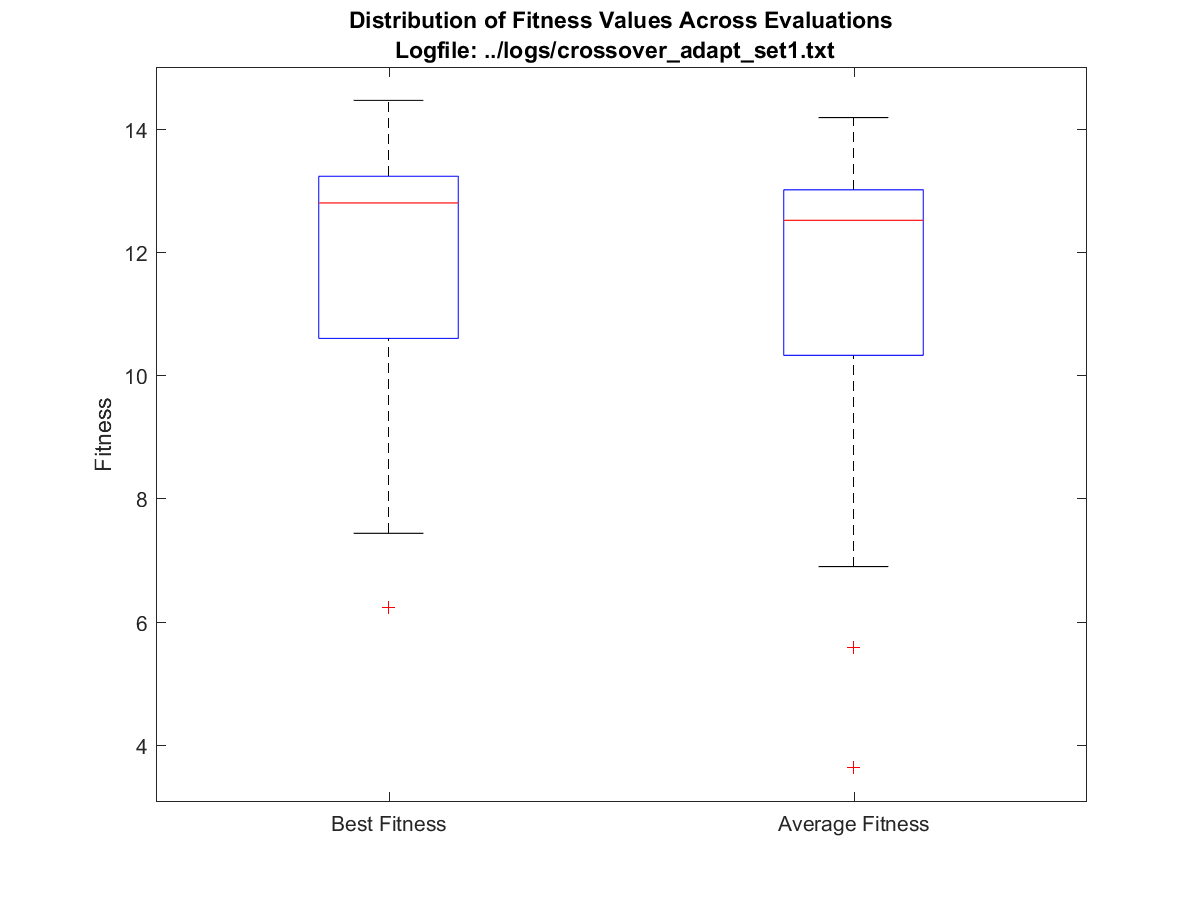
\includegraphics[width=3.25in]{assn1c_boxplot_crossover_adapt_set1.png}
  \captionof{figure}{Adaptive Crossovers, 50Shapes.txt}
  \label{fig:boxplot1}
\end{minipage}%
\begin{minipage}{.5\textwidth}
  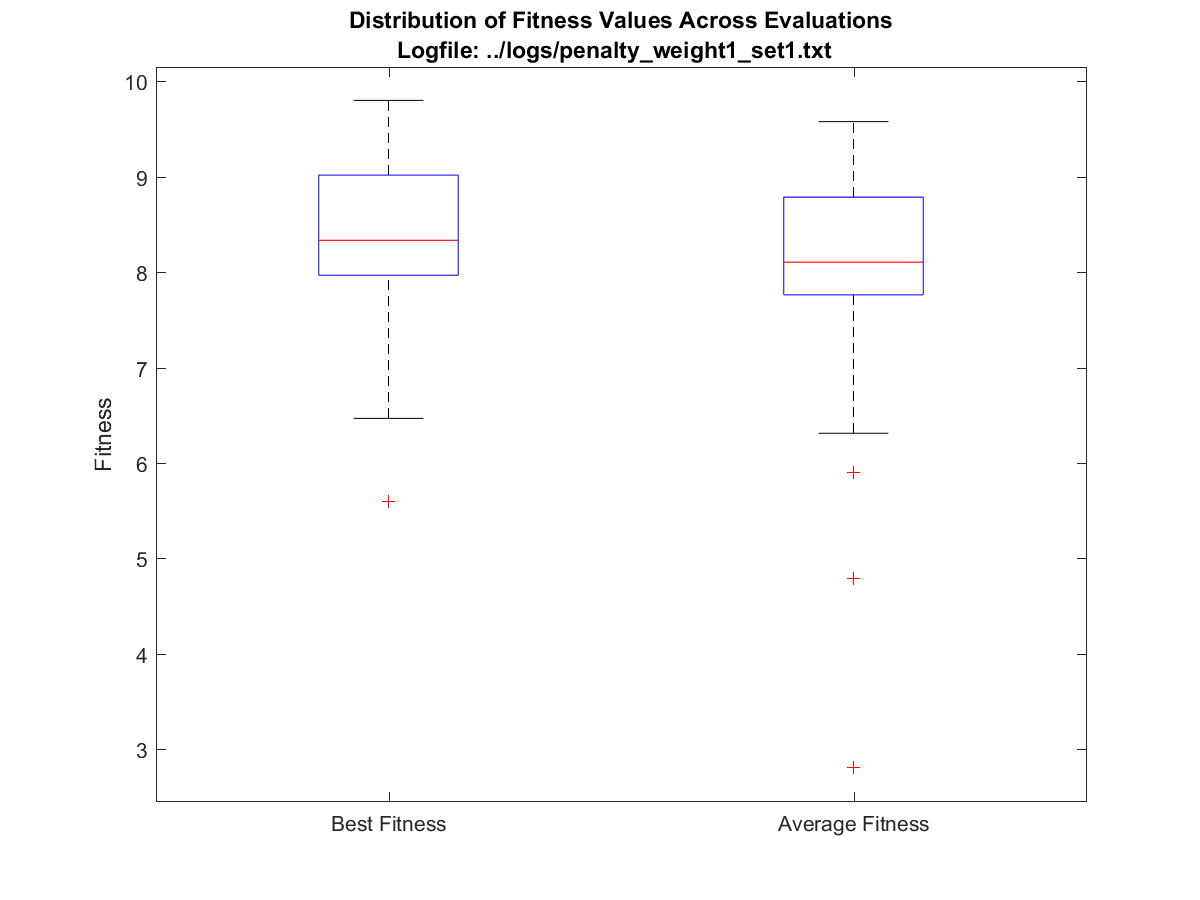
\includegraphics[width=3.25in]{assn1c_boxplot_penalty_weight1_set1.png}
  \captionof{figure}{Penalty Weight 1.0, 50Shapes.txt}
  \label{fig:boxplot2}
\end{minipage}
\end{figure}

\begin{figure}[h]
\centering
\begin{minipage}{.5\textwidth}
\centering
  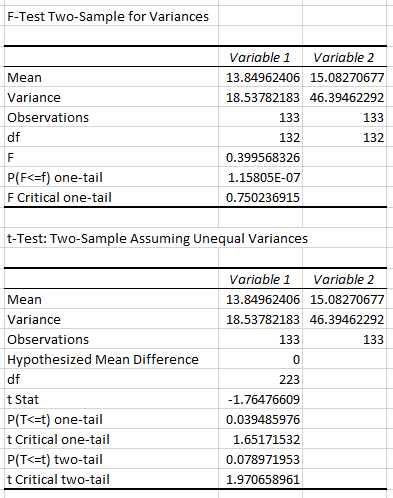
\includegraphics[width=2.5in]{assn1c_stat_anal_crossovers_set1.png}
  \captionof{figure}{Adaptive Crossovers, 50Shapes.txt}
  \label{fig:statanal1}
\end{minipage}%
\begin{minipage}{.5\textwidth}
\centering
  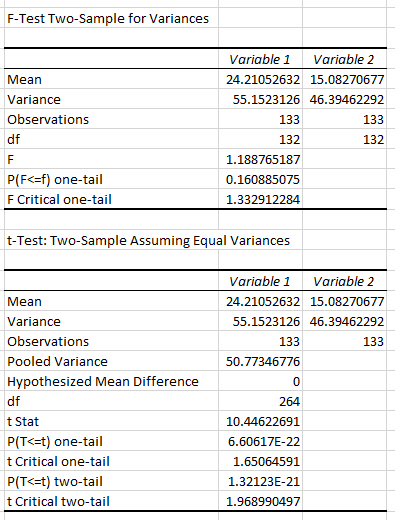
\includegraphics[width=2.4in]{assn1c_stat_anal_penalty_weight_1_set1.png}
  \captionof{figure}{Penalty Weight 1.0, 50Shapes.txt}
  \label{fig:statanal2}
\end{minipage}
\end{figure}


\section{Bonus 1}\label{sect:bonus1}

The self-adaptivity aspect was further tested. Three methods were implemented: fixed penalty weight, time-scaling penalty weight, and self-adaptive penalty weight. For this test, the fixed penalty weight was set at 2.0 and the time-scaling scaled to a maximum of 10.0.

The results show that there really was no great improvement on one method verses the other. Both the fixed and self-adaptive penalty methods remained at mostly the same average best value. It is interesting to note the the time-scaling approach underperformed on the 50Shapes data set and performed quite well on the 100ShapesComplex data set. In the more complex data set, allowing the algorithm to be more exploratory in the early evaluations seems to prove beneficial.

\begin{figure}[h]
\begin{minipage}{.5\textwidth}
  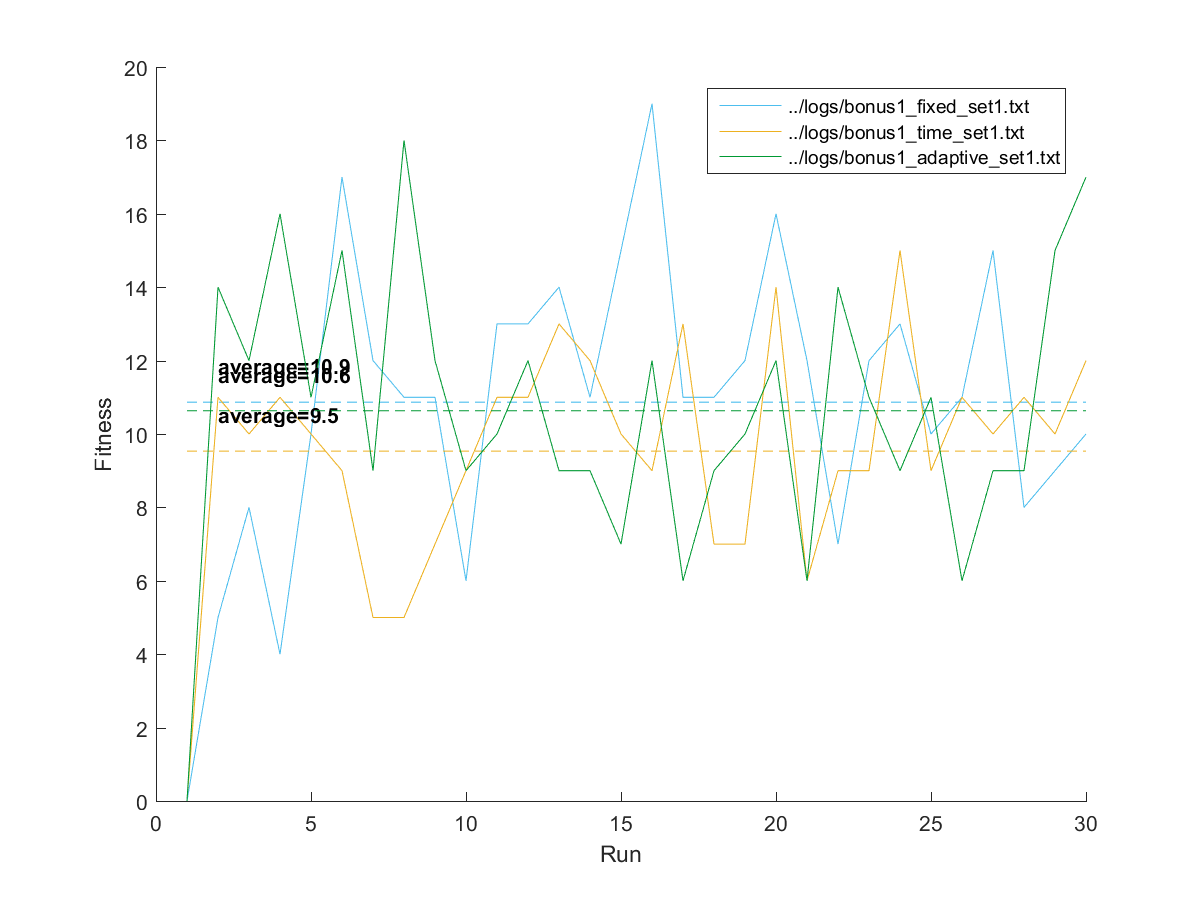
\includegraphics[width=3.25in]{assn1c_bonus1_set1.png}
  \captionof{figure}{Penalty Methods, 50Shapes.txt}
  \label{fig:bonus2_1}
\end{minipage}%
\begin{minipage}{.5\textwidth}
\centering
  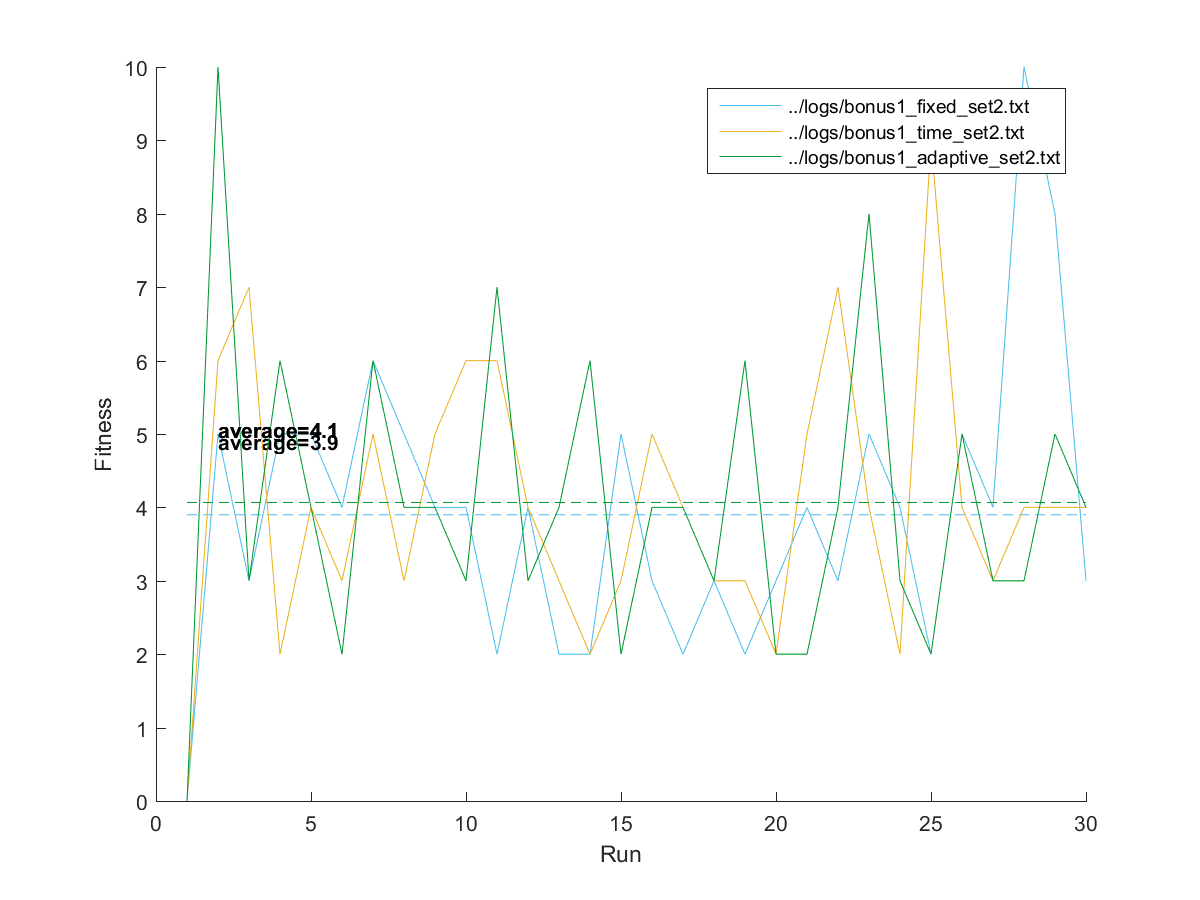
\includegraphics[width=3.25in]{assn1c_bonus1_set2.png}
  \captionof{figure}{Penalty Methods, 100Shapes.txt}
  \label{fig:bonus2_2}
\end{minipage}
\end{figure}
\begin{figure}[h]
	\centering
  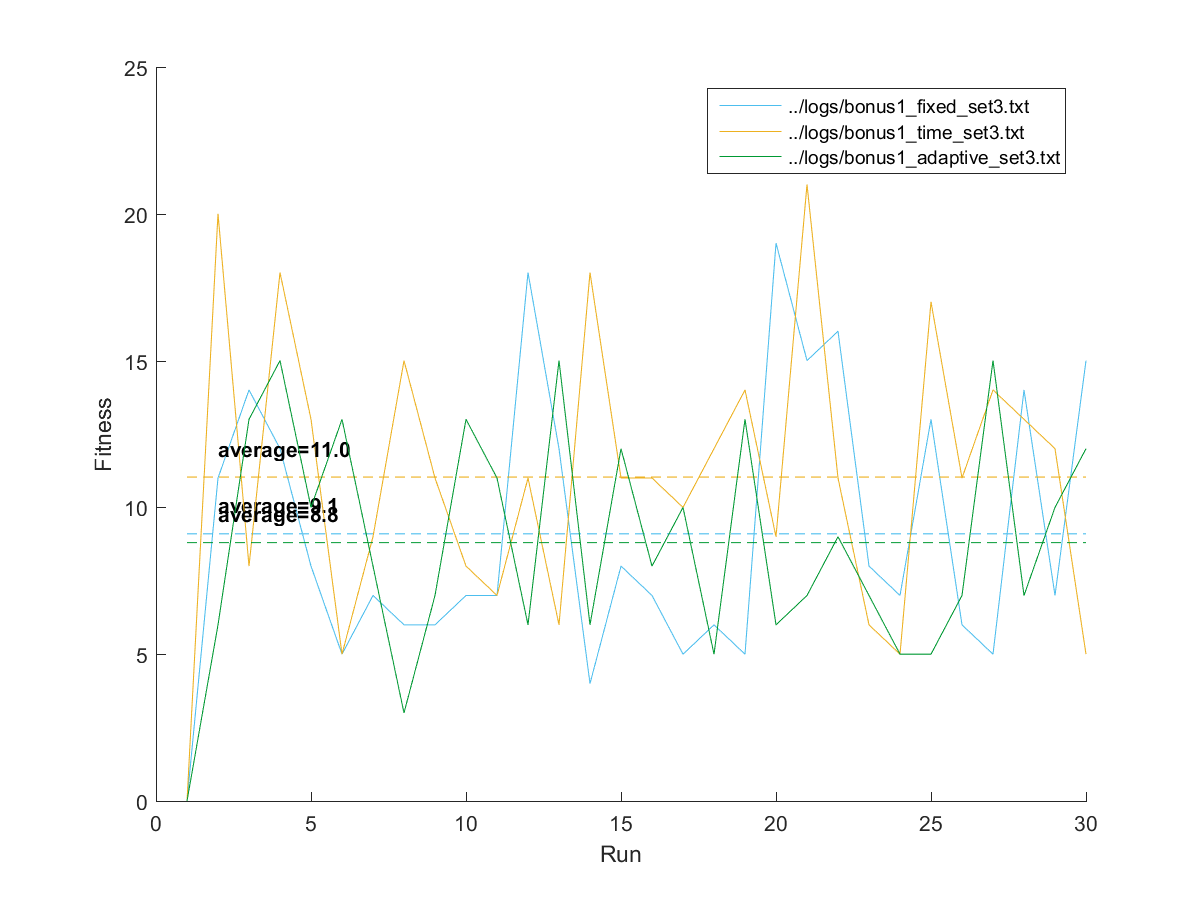
\includegraphics[width=3.25in]{assn1c_bonus1_set3.png}
  \captionof{figure}{Penalty Methods, 100ShapesComplex.txt}
  \label{fig:bonus2_3}
\end{figure}

\section{Bonus 2}\label{sect:bonus2}

To further test self-adaptability, the mutation rate was set to be adaptable. For offspring created, there was an equivalent random chance of inheriting each parent's mutation rate. Additionally, \textit{n} had a small chance to mutate (equivalent to the genetic mutation rate) by $\pm$1 2\%. For analysis, the mutation rate was averaged across all member of the population for each generation and then logged. The test parameters were kept exactly the same as in Section \ref{sect:selfadaptive}.

These graphs are a little more difficult to interpret, as there are now many factors influencing the results. As shown in Figures \ref{fig:bonus2_1}, \ref{fig:bonus2_2}, and \ref{fig:bonus2_3} all the averages are fairly clustered together. It is also worth noting that some of the results here actually contradict the results obtained in Section \ref{sect:selfadaptive}, that is, the control scored better than the adaptive crossovers alone. This seems to be due to randomness, as both averages are valued fairly close to each other. This trend is also not consistent across all three data sets.

Interestingly enough, there is a clear improvement for the combined adaptive parameter for the 100Shapes data set, and a slight improvement for the 100ShapesComplex data set. It seems that the allowing both parameters to adapt has allowed the algorithm to better exploit the more varied fitness landscape provided by the more complex data sets.

Similar to the finding in Section \ref{sect:selfadaptive}, there was not clear trend in the direction that the adaptive parameters took. For both crossovers and mutation rate, some runs increased the values and some decreased. Again, this can be seen in detail by examining the logs located in the ./logs/ directory) shows no consistent trend. Once again, it can be assumed that each run's random initialization took it to a different area of the fitness landscape where more or less of each parameter was more desirable.

\begin{figure}[h]
\begin{minipage}{.5\textwidth}
  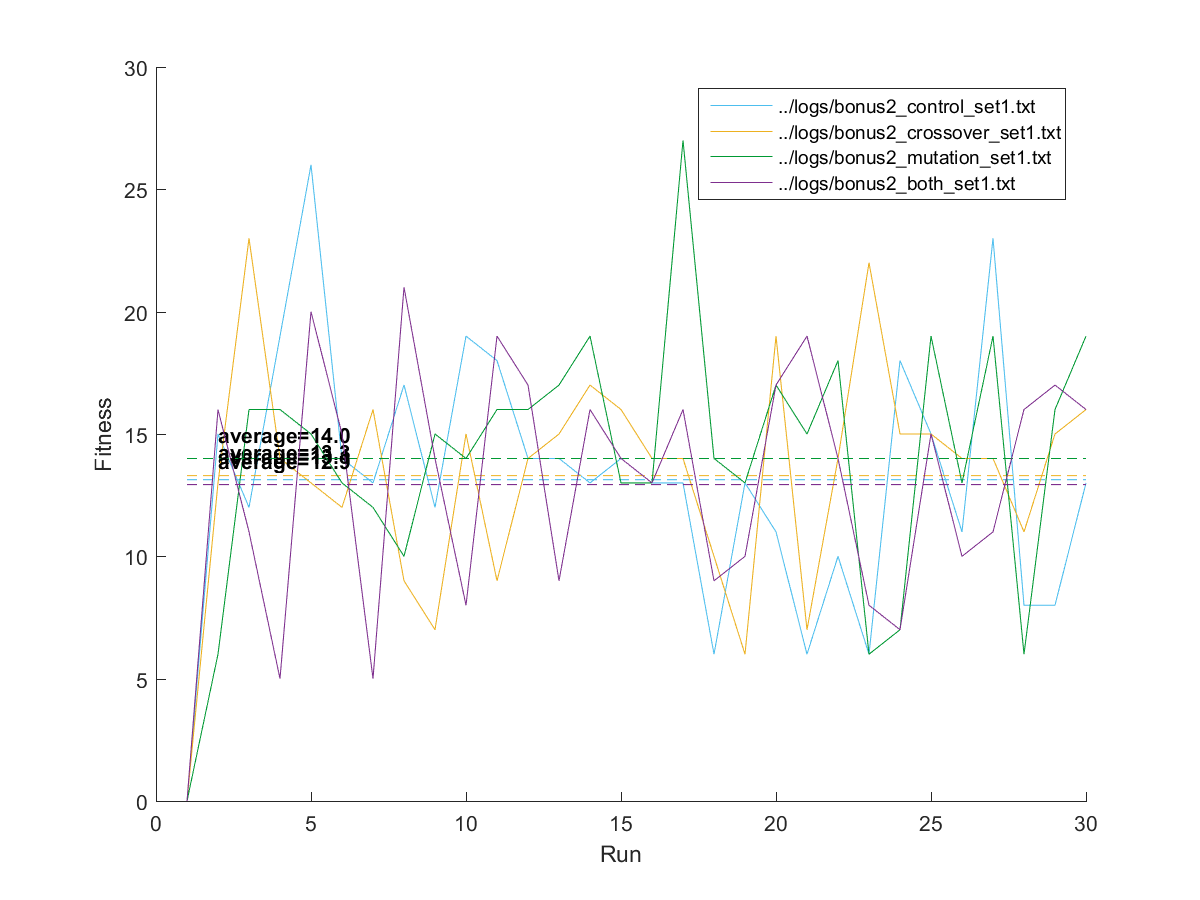
\includegraphics[width=3.25in]{assn1c_bonus2_set1.png}
  \captionof{figure}{Adaptive, 50Shapes.txt}
  \label{fig:bonus2_1}
\end{minipage}%
\begin{minipage}{.5\textwidth}
\centering
  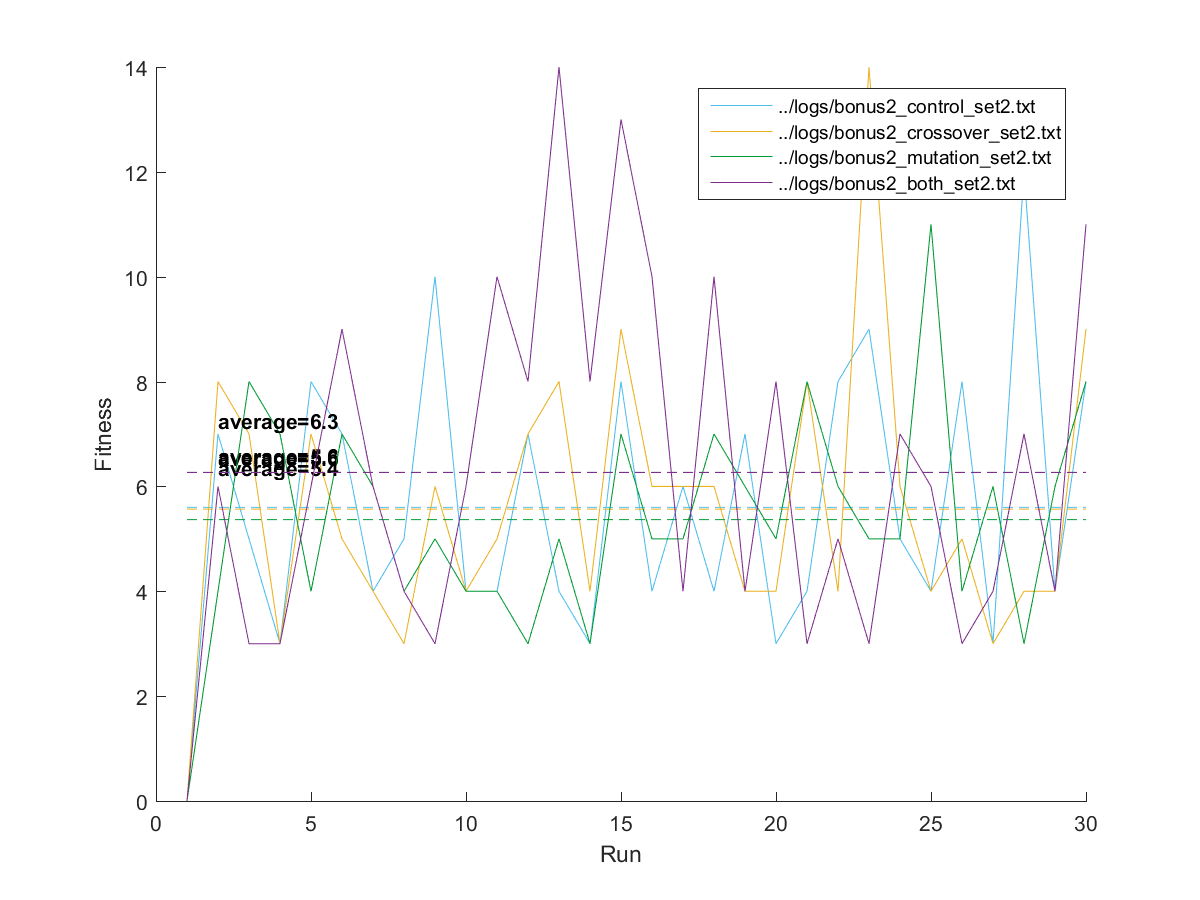
\includegraphics[width=3.25in]{assn1c_bonus2_set2.png}
  \captionof{figure}{Adaptive, 100Shapes.txt}
  \label{fig:bonus2_2}
\end{minipage}
\end{figure}
\begin{figure}[h]
	\centering
  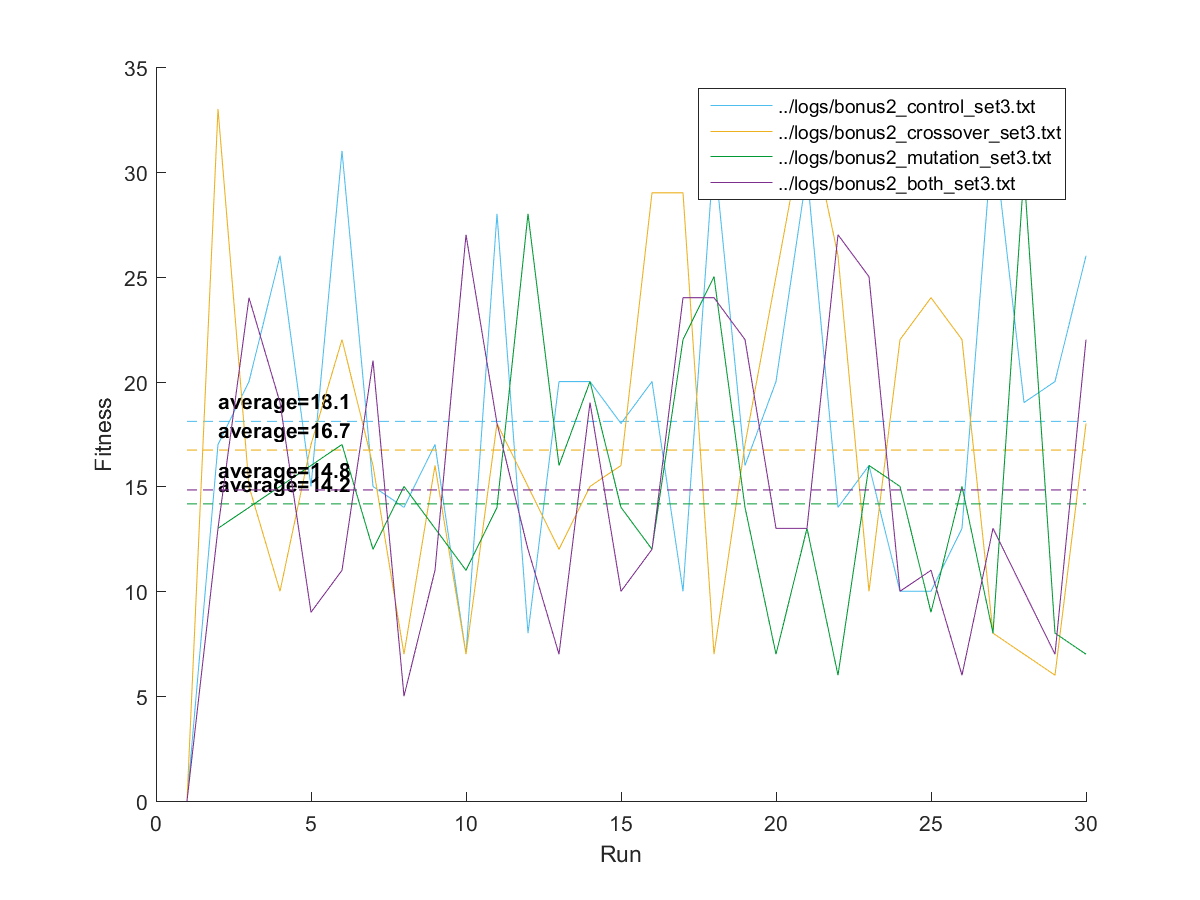
\includegraphics[width=3.25in]{assn1c_bonus2_set3.png}
  \captionof{figure}{Adaptive, 100ShapesComplex.txt}
  \label{fig:bonus2_3}
\end{figure}

\section{Addendum}
As a proof that the self-adaptive penalty function works, this graph has been included. Here, the author forgot to add a check to stop the penalty function from going negative. Since the fitness was calculated by subtracting weighted penalty value, negative weights allowed the fitness to skyrocket. See Figure \ref{fig:addendum}.

\begin{figure}[h]
	\centering
  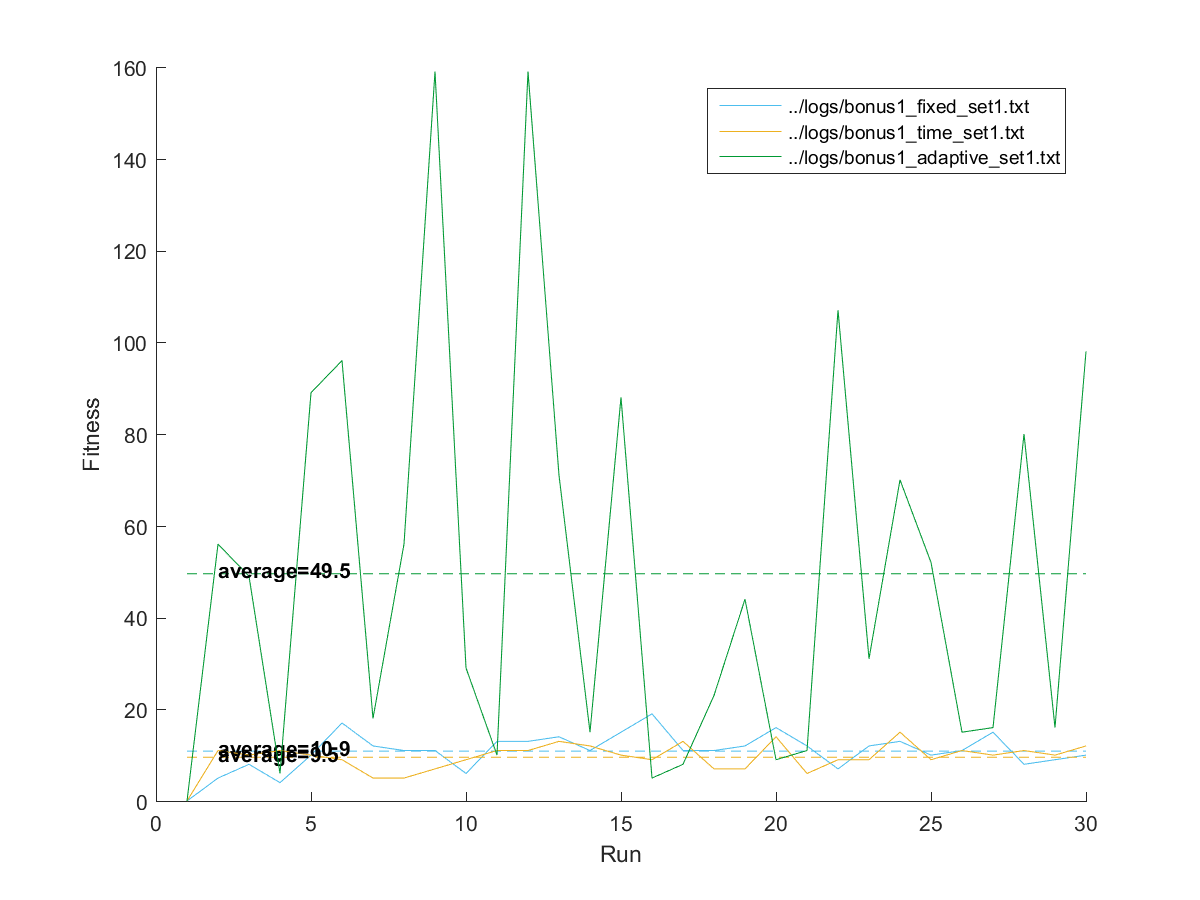
\includegraphics[width=3.25in]{assn1c_bonus1_negative_weights.png}
  \captionof{figure}{Adaptive, 100ShapesComplex.txt}
  \label{fig:addendum}
\end{figure}

\end{document}